\chapter{递推、非平衡序与伊辛自旋}

\lectureoverview{从房间的一半释放出来的气体会迅速趋向平衡，然而可逆力学表明，足够长的演化也必定会产生向那个例外状态的回归。我们根据相空间体积估计回归时间，把递推与宇宙那个无法解释的低熵开端区分开来，并利用由此产生的谜题来讨论玻尔兹曼大脑、连贯的历史，以及由能量流维持的生命。随后我们转向磁序。独立的两态自旋给出一个可精确求解的热身例子：组合学决定了配分函数，而磁化强度是一个双曲正切。近邻相互作用最终恢复上--下对称性，并引出一维伊辛模型。}

\section{一屋子最终会回归的空气}

从房间左半边的所有空气开始。人们可以用一块隔板来制备这个状态：把右半边抽成真空，把空气放在左边，然后抽掉隔板。气体迅速扩散到整个房间并趋近热平衡。熵增加。没有发生任何令人惊讶的事情。

现在把房间密封起来并等待。连续一百万次正面朝上是一份极不可能的抛硬币记录，但一个无限重复的实验最终会产生极不可能的记录。同样的逻辑适用于气体。在某个遥远的时刻，它的所有分子将再次被发现位于左半边，或者位于某个同样特殊的区域。这样的回归就是庞加莱递推。

精确的定理比这幅图像要稍微谨慎一些。对于一个测度有限、其动力学保持相空间体积的相空间区域，几乎每一个初始点都会任意接近地回到它的出发点。像\emph{所有分子都在左半边}这样的宏观陈述则更容易：它只要求轨迹重新进入一个有限的粗粒化区域，而不要求每一个分子坐标都精确回归。实际的问题是这需要多长时间。

\subsection{一个高维相点}

对于\(N\)个经典粒子，相空间有\(6N\)个坐标，\begin{equation}
 \Gamma=(\bm x_1,\ldots,\bm x_N;\bm p_1,\ldots,\bm p_N).
 \label{eq:sm8-phase-point}
\end{equation}
位置受房间限制。在总能量固定时，动量也受到限制，因为一个粒子不可能携带任意大的动量而不携带任意大的能量。因此，在递推论证的假设下，允许的能量壳层具有有限的测度。

相点确定性地运动，但在多体气体中它的运动是混沌的。邻近的轨迹迅速分离，就像在一连串台球碰撞中那样。经过粗粒化之后，一条很长的轨迹看起来在可及区域内到处游荡。

\begin{figure}[t]
\centering
\includegraphics[width=0.90\textwidth]{lecture_08_figure_02.png}
\caption{一个示意性的相空间区域以及在其中游荡的复杂轨迹。这幅图被有意画成低维的；真实的气体生活在一个\(6N\)维空间中。}
\lectureframe{00:06:41}
\end{figure}

这幅低维草图立刻诱使我们犯一个错误。如果那个特殊状态占据了所画矩形的一半，人们可能会说气体应该有半数时间待在那里。但是\emph{每个分子都位于左半边}约束了每一个位置坐标，而不只是相点的一个坐标。

只取在一维空间中运动的两个粒子，坐标分别为\(x_1\)和\(x_2\)。它们的位形空间是一个正方形。要求\(x_1<L/2\)选出正方形的一半；同时要求\(x_1<L/2\)和\(x_2<L/2\)则选出一个四分之一：
\begin{equation}
 P_2=\frac{1}{2}\frac{1}{2}=\frac{1}{4}.
 \label{eq:sm8-two-particle-quarter}
\end{equation}

\begin{figure}[t]
\centering
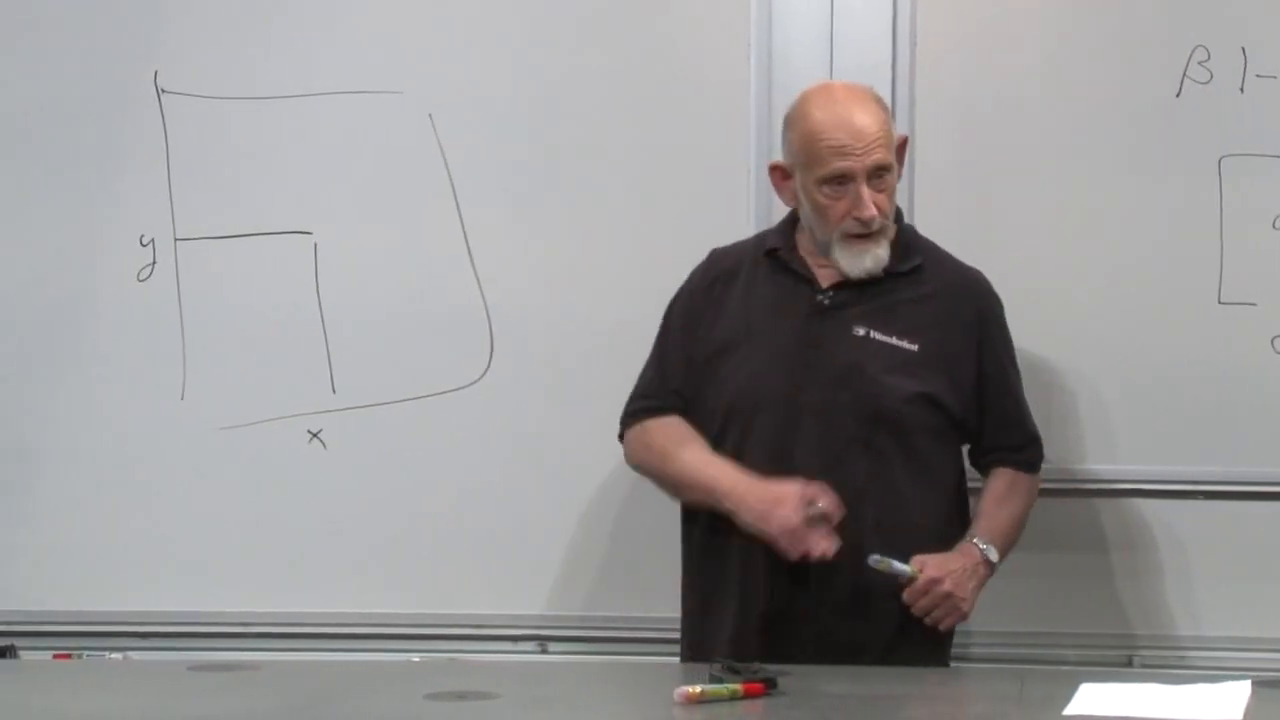
\includegraphics[width=0.90\textwidth]{lecture_08_figure_07.png}
\caption{对于两个一维粒子，较小的正方形代表两个坐标都位于房间所选那一半中的位形。}
\lectureframe{00:07:08}
\end{figure}

三个粒子给出\(1/2^3\)，而\(N\)个粒子给出
\begin{equation}
 P_{\mathrm{half}}(N)
 =\left(\frac{1}{2}\right)^N.
 \label{eq:sm8-half-probability}
\end{equation}
指数就是全部要点。一个二分之一因子很平常；二分之一的一个宏观粒子数次幂则超出了平常的直觉。

\begin{classroomqa}
\audiencequestion{答案难道不应该是\(1/3^N\)吗，因为分子还有其他空间方向？}
\lecturerresponse{这取决于所施加的条件。如果唯一的问题是每个粒子是否都位于分隔墙的左侧，那么每个粒子满足一个二元条件，答案就是\(2^{-N}\)。如果再约束其可用位置空间中另一个独立的分数，就会再提供一个因子。
\lecturetimestamp{00:07:47--00:08:05}}
\end{classroomqa}

\section{相体积、熵与递推尺度}

同一个估计也可以不借助“一半”来写出。设房间具有普通空间体积\(V\)，并设\(v\)为一个较小的区域，我们要求在其中找到每一个分子。忽略两个宏观态共有的动量因子后，可用的位形空间体积为
\begin{equation}
 \Omega_{\mathrm{room}}\propto V^N,
 \qquad
 \Omega_{\mathrm{small}}\propto v^N.
 \label{eq:sm8-config-volumes}
\end{equation}
因此，长时间中处于小宏观态的比例为
\begin{equation}
 P(v)
 =\frac{\Omega_{\mathrm{small}}}{\Omega_{\mathrm{room}}}
 =\left(\frac{v}{V}\right)^N.
 \label{eq:sm8-volume-ratio}
\end{equation}

\begin{figure}[t]
\centering
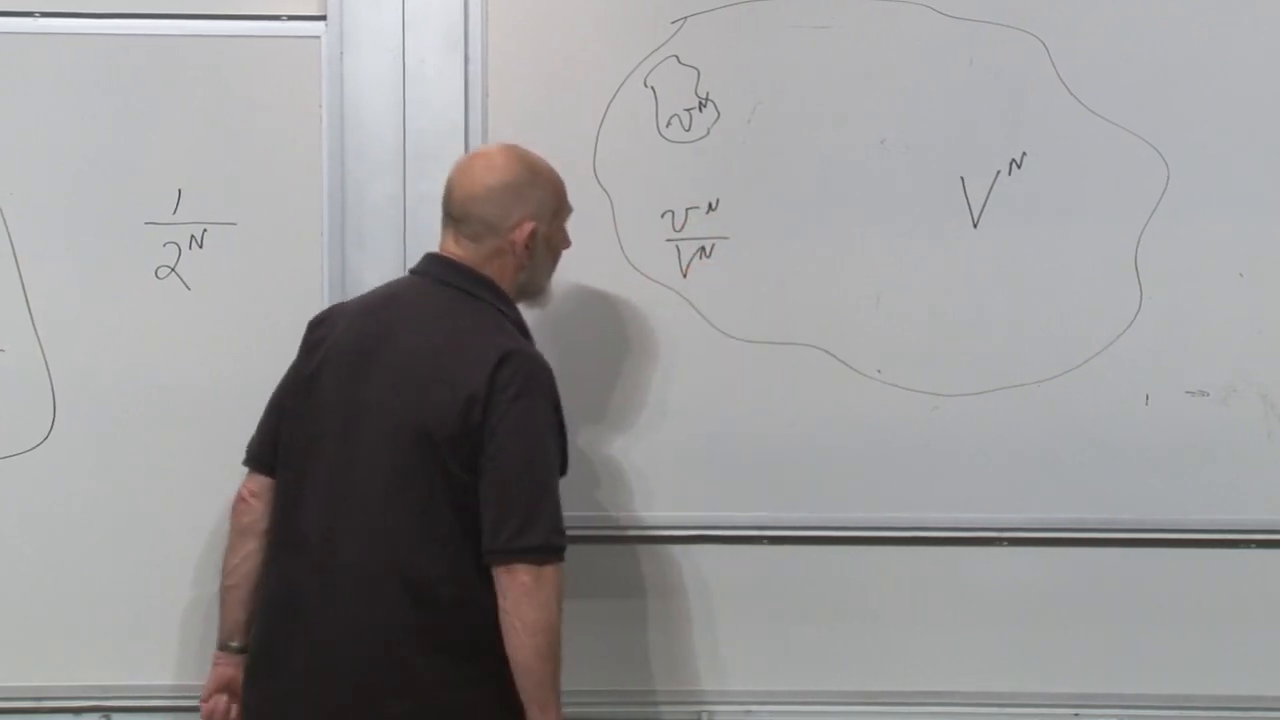
\includegraphics[width=0.90\textwidth]{lecture_08_figure_08.png}
\caption{黑板上的普遍相体积图像：可及区域\(V^N\)内部的一个小区域\(v^N\)，其比值为\(v^N/V^N\)。}
\lectureframe{00:10:44}
\end{figure}

在\(k_B=1\)的单位制下，熵是可及相体积的对数。若\(S_A=\log\Omega_A\)是受约束宏观态的熵，而\(S_{\rm eq}=\log\Omega_{\rm eq}\)是平衡态的熵，则
\begin{equation}
 \begin{aligned}
 P(A)
 &=\frac{\Omega_A}{\Omega_{\rm eq}}\\
 &=\exp\!\left(S_A-S_{\rm eq}\right)\\
 &=e^{-\Delta S},\\
 \Delta S&=S_{\rm eq}-S_A.
 \end{aligned}
 \label{eq:sm8-entropy-probability}
\end{equation}
对于半房间态，\(\Delta S=N\log 2\)，而\eqref{eq:sm8-entropy-probability}恰好化为\(2^{-N}\)。简写\(P\sim e^{-S_{\rm eq}}\)仅在把特殊区域的熵当作固定参考时才适用；具有物理意义的指数是熵亏损\(\Delta S\)。

\begin{classroomqa}
\audiencequestion{这是位形空间的体积，而不是整个相空间的体积吗？}
\lecturerresponse{对于这一比较而言，是的。我们施加的是位置条件，同时让动量分布保持在同一温度，因此共同的动量空间因子相消。完全一般的复现陈述使用相空间；而这个特定的概率可以由位形空间比值算出。
\lecturetimestamp{00:11:21--00:11:40}}
\end{classroomqa}

假设系统在微观关联时间或混合时间\(\tau_{\rm mix}\)上失去对其详细位置的记忆。那么，概率为\(P(A)\)的稀有区域会在如下尺度上被遇到：
\begin{equation}
 \tau_{\rm rec}
 \sim \frac{\tau_{\rm mix}}{P(A)}
 \sim \tau_{\rm mix}e^{\Delta S}.
 \label{eq:sm8-recurrence-time-general}
\end{equation}
对于半房间条件，
\begin{equation}
 \tau_{\rm rec}\sim\tau_{\rm mix}2^N.
 \label{eq:sm8-recurrence-time-half}
\end{equation}
讲座使用了刻意粗略的房间尺度估计\(N\sim10^{30}\)，给出令人难忘的尺度
\(\tau_{\rm rec}/\tau_{\rm mix}\sim2^{10^{30}}\)。在普通大气密度下，一个房间更接近\(10^{27}\)个分子，但把\(10^{30}\)换成\(10^{27}\)不会改变任何结论：复现时间仍然比宇宙年龄大得无法想象。

\begin{classroomqa}
\audiencequestion{复现时间以什么单位测量？从秒改成小时，或改成一个极短的单位，会改变结论吗？}
\lecturerresponse{量纲前因子是\(\tau_{\rm mix}\)；巨大的数是无量纲比值\(\tau_{\rm rec}/\tau_{\rm mix}\)。把秒改成小时只是除以一个普通的换算因子，与\(2^{10^{30}}\)相比可以忽略。单次访问角落的持续时间确实取决于分子速率。这个估计关心的是这种访问多么罕见地开始。还存在量子复现定理，但这里不需要它。
\lecturetimestamp{00:17:24--00:19:18}}
\end{classroomqa}

\begin{classroomqa}
\audiencequestion{计算一个任何实验都不可能等待的时间，目的何在？}
\lecturerresponse{要点是概念性的。它告诉我们，封闭的力学系统在何种意义上保持可逆。它几乎全部时间都待在平衡态附近，但在足够长的尺度上，它也会向低熵方向发生涨落。因此，第二定律是一个关于特殊初始数据的、概率上压倒性的陈述，而不是一条禁止反向运动的微观方程。
\lecturetimestamp{00:15:12--00:16:35}}
\end{classroomqa}

\section{可逆性与特殊的开端}

有意地从微小的半房间区域出发。几乎每一条邻近轨道都会立刻离开它，因为外面的相体积远多于里面。气体迅速扩散，然后等待极长的时间才返回。快速弛豫与漫长等待之间的这种不对称并不违反可逆力学。

快速逃逸的时间反演并不是整个等待期。它是短暂且协调得不可思议的一段过程：看起来处于平衡的分子速度恰好自行安排，使气体\emph{嗖地}冲进房间的一半。在普通逃逸结束时把每个动量都反向，气体就会反向重演逃逸过程。漫长的等待时间，就是那种特殊的入射速度模式自发出现所需的时间。

\begin{classroomqa}
\audiencequestion{时间对称性是否意味着缓慢复现到角落所需的时间，与最初从那里逃逸所需的时间一样长？}
\lecturerresponse{不是。把逃逸与其精确的时间反演相比较。两者都很快。花费巨大时间的是在平衡态中等待那个引发反向嗖地冲入的精确入射涨落。在极其漫长的记录中，偏离平衡的远足会沿两个时间方向发生，其局部历史是对称的。
\lecturetimestamp{00:20:46--00:21:58}}
\end{classroomqa}

因此，复现论证只能解释时间箭头的一部分。它解释了为什么在系统始于低熵区域的\emph{给定条件}下，熵通常会上升。它并不解释为什么初始条件是特殊的。在宇宙学中，这个缺失的前提变成了核心问题：为什么可观测宇宙会始于其引力相空间中如此异常小的一个区域？

\begin{classroomqa}
\audiencequestion{复现是否适用于宇宙学？在宇宙扩散开来之后，如果等待足够久，它是否可能复现？}
\lecturerresponse{这个问题无法回避，但其答案取决于整体宇宙学。一个真正封闭、具有有限平衡态空间的系统会倾向于复现。膨胀的时空、引力、视界，以及无限或非定常的状态空间，都可能改变前提。这里重要的教训更为狭窄：仅凭平衡态复现图景，并不足以对我们所看到的这个有结构的宇宙给出令人满意的统计解释。
\lecturetimestamp{00:19:59--00:20:45}}
\end{classroomqa}

\begin{classroomqa}
\audiencequestion{复现是否依赖于一开始把气体制备在一个小区域中？如果房间从平衡态开始，空气最终仍然会聚集到一个角落吗？}
\lecturerresponse{会。复现涉及封闭系统的长时间动力学，因此一个看起来处于平衡态的初始态也会经历罕见的低熵涨落。制备半房间状态之所以重要，是出于另一个原因：它让我们能够以已知的特殊初始状态为条件，并追问为什么熵在此后立即上升。
\lecturetimestamp{00:22:04--00:22:20}}
\end{classroomqa}

\section{为什么随机涨落所预言的东西太少}

人们可能会试图把复现变成一种宇宙学：也许宇宙几乎全部永恒时间都处于平衡态，而我们当前的世界是一次罕见的涨落。这个提议未能通过一项尖锐的统计检验。以观察者的存在为条件，然后追问该观察者还应当预期看到什么。

大到足以形成一个行星的涨落极其罕见。形成两个行星的涨落需要更大的熵亏缺，因而更加罕见。形成恒星、星系、宇宙微波背景，以及关于漫长过去且彼此一致的记录的涨落，则还要罕见得多，多出一个巨大的额外指数因子。因此，平衡态涨落理论预言的是足以供观察的最小涨落，而不是实际观察到的这个丰富而连贯的世界。在其最极端的形式中，最小的观察者被称为玻尔兹曼大脑。

其逻辑是条件概率。令\(A\)表示发生一次观察者尺度涨落的事件，\(B\)表示一个独立的第二结构。如果二者都具有微小概率\(p\)，那么
\begin{equation}
 P(B\mid A)=p,
 \qquad
 P(A\cap B)=p^2.
 \label{eq:sm8-conditional-fluctuations}
\end{equation}
得知第一次涨落已经发生，并不会使第二次涨落变得可能。彩票类比在这个层面上是精确的：先前的中奖者在下一次独立抽奖中并没有更高的机会。因此，观察者可以以自身存在为条件，但仍然应当惊讶地发现自己身处一个独立地具有结构的环境之中。

\begin{classroomqa}
\audiencequestion{既然一个行星或一个玻尔兹曼观察者已经存在，另一个的概率真的更小吗？}
\lecturerresponse{第二个独立罕见涨落的条件概率仍是同一个微小的一次事件概率，而不是它的平方。二者同时发生的联合概率才是平方。这正是为什么第一个观察者仍应预期自身之外是热无序的。发现一个配偶、另一个行星，以及一片有序的天空，都是反对如下前提的证据：该观察者是由一次孤立的平衡态涨落组装而成的。
\lecturetimestamp{00:26:12--00:30:27}}
\end{classroomqa}

\subsection{关于过去的连贯记录}

同样的论证也适用于历史。两本彼此一致的教科书、符合同一膨胀历史的天文记录、地质地层、记忆和实验室笔记本，都会彼此约束。一本随机出现的教科书可以包含任何故事。而一整套关于同一过去且彼此一致的记录网络，则占据一个小得多的相空间区域。

课堂例子使用了那个熟悉的传说：乔治·华盛顿砍倒了一棵樱桃树。这个传说是否真实无关紧要。要点在于，在一个于当前瞬间涨落而存在的世界中，一本书中的句子并没有给出任何动力学理由，使另一条记录与它一致。连贯的关联是共同历史的证据，而不仅仅是一次瞬时意外的证据。

\begin{classroomqa}
\audiencequestion{这里的\emph{历史一致性}是什么意思？}
\lecturerresponse{它意味着，当前的许多记录作为共同过去的后果而彼此吻合。涨落可以伪造记录和记忆，但伪造一个相互一致的网络所需的涨落，要比伪造一个最小观察者大得多。因此，复现理论预言，大多数类似观察者的涨落并不具备我们实际发现的那种一致性。
\lecturetimestamp{00:30:30--00:31:12}}
\end{classroomqa}

\begin{classroomqa}
\audiencequestion{宇宙是否仍可能是一个封闭系统，只不过其平衡化时间和复现时间极其漫长？}
\lecturerresponse{这种可能性并不能消除统计问题。在无限漫长的历史中，会出现许多类似观察者的涨落，而其中绝大多数都是没有一致周围历史的最小涨落。从那个系综中选出的一个观察者，不应期望看到我们的观测结果。因此，宇宙学家把玻尔兹曼大脑问题当作对宇宙学测度和晚期模型的检验来认真对待，而不是把它当作复现已经被观测到的断言。
\lecturetimestamp{00:31:13--00:32:42}}
\end{classroomqa}

\section{作为由流动维持的结构之生命}

生命似乎提出了相反的困难。有机体在长时间内维持着精巧的组织；它们看起来不像短暂的偶然涨落。解决之道在于，第二定律适用于完整的封闭系统。一个子系统可以降低或维持其熵，只要其环境中发生更大的熵增：
\begin{equation}
 \dot S_{\rm total}
 =\dot S_{\rm subsystem}+\dot S_{\rm environment}\geq 0.
 \label{eq:sm8-open-system-second-law}
\end{equation}

地球并不处于热平衡。在人类的时间尺度上，它近似是定常的，但定常并不意味着静止。能量流经它。阳光到达，经过许多过程被降级，并以较低的有效温度辐射出去。这种流通可以在总熵上升的同时维持局部的组织。

水流过管道提供了最直接的力学图像。流动中可以包含持续存在的涡旋和旋涡。它们是有组织的结构，但它们由水流维持。把两端封住，停止流动，随着水趋近于沉闷的平衡，黏性会抹去这些涡旋。流出的水比流入的水更暖，因此更大的系统已经支付了熵的账单。

\begin{classroomqa}
\audiencequestion{生命会降低熵吗？为什么它的组织能够持续存在，而不是像普通涨落那样出现又消失？}
\lecturerresponse{生命可以在局部维持或降低熵，但只能通过输出更多的熵来实现。它的持续存在来自一种定常的非平衡流动，主要是太阳能流经地球的流动。如果地球对入射和出射辐射都是封闭的，它最终会趋近热平衡，而有组织的活动将会停止。生命更接近于溪流中的一个涡旋，而不是一个平衡涨落。
\lecturetimestamp{00:32:43--00:35:42}}
\end{classroomqa}

至此，我们离开\emph{有趣的东西}，并回到讲座中刻意平淡的说法：某种乏味的东西——磁体。

\section{冷却磁体：磁畴与一个被选定的方向}

统计力学常常把一个数学模型称为磁体，即使它并不是一块字面意义上的铁。有用的共同特征是，一组能够发生有序化的局域自由度。在真实的磁性材料中，这些自由度可能来自原子磁矩、电子自旋、轨道电流或晶体单元的有效磁矩。

在高温下，热无序使局域磁矩指向许多方向，从而给出很小或没有净磁化。如果相邻磁矩在排列一致时能量更低，那么冷却就允许小的排列一致的磁畴形成。进一步冷却使能量优势更加重要，关联磁畴随之长大。在支持铁磁相变的系统中，关联长度在有限的临界温度处变为宏观尺度。于是，有序相会选择一个取向，尽管零场能量事先并不偏好某一个取向。

\begin{classroomqa}
\audiencequestion{微观磁体是否应当因为北极吸引南极而倾向于反向排列？}
\lecturerresponse{有效相互作用取决于材料。普通的偶极子直觉并不是整个微观问题；交换作用、晶体结构和相互竞争的相互作用都很重要。铁磁材料是那些有效低能倾向有利于平行排列的材料，而其他材料则可能有利于反向排列。
\lecturetimestamp{00:39:56--00:40:30}}
\end{classroomqa}

\begin{classroomqa}
\audiencequestion{为了使磁矩排列整齐，材料冷却时是否必须存在外磁场？}
\lecturerresponse{不需要。相互作用无需磁场即可产生有序。在完全对称的理想化情形中，不同方向在能量上等价，因此实际实现的方向由初始涨落、边界或任意小的杂散场选定。从这些等价方向中选定一个，就是自发对称破缺；宏观有序的出现就是磁性相变。
\lecturetimestamp{00:40:31--00:42:33}}
\end{classroomqa}

真实材料很复杂，因此我们现在做极端的简化。每个局域磁矩只能向上或向下：
\begin{equation}
 \sigma_i=+1\quad\hbox{or}\quad\sigma_i=-1.
 \label{eq:sm8-ising-spin}
\end{equation}
这个模型中没有东或西。两个允许的取向是模型的定义，正如正面和反面是抛硬币的两个结果。其价值不在于微观真实性，而在于数学上的清晰性，以及它能够表示许多系统共有的有序化现象。

\begin{classroomqa}
\audiencequestion{这两个态的对象在物理上是什么？应该把它们想象成粒子吗？}
\lecturerresponse{可以想象晶体格点上的原子，每个原子具有由自旋或微观电流产生的有效磁矩。然而，对于这个模型而言，只有这个二值变量才是重要的。限制为向上和向下，是为了使统计力学变得简单。
\lecturetimestamp{00:44:22--00:45:01}}
\end{classroomqa}

\section{外场中的独立自旋}

第一个模型包含\(N\)个彼此不相互作用的自旋。外场\(H\)提供了唯一的能量尺度，而\(\mu\)衡量一个自旋与其耦合的强度。我们保留计算中使用的符号约定：
\begin{equation}
 \epsilon_i=\mu H\sigma_i.
 \label{eq:sm8-single-spin-energy}
\end{equation}
对于\(H>0\)，向上自旋\(\sigma_i=+1\)的能量为\(+\mu H\)，而向下自旋\(\sigma_i=-1\)的能量为\(-\mu H\)。因此，这一约定使正场有利于向下自旋。它与另一种常见的命名约定相反，但只要符号使用一致，物理就不依赖于名称。

设\(n\)为向上自旋的数目，\(m\)为向下自旋的数目。则
\begin{equation}
 n+m=N,
 \qquad
 E=(n-m)\mu H.
 \label{eq:sm8-counting-energy}
\end{equation}

\begin{figure}[t]
\centering
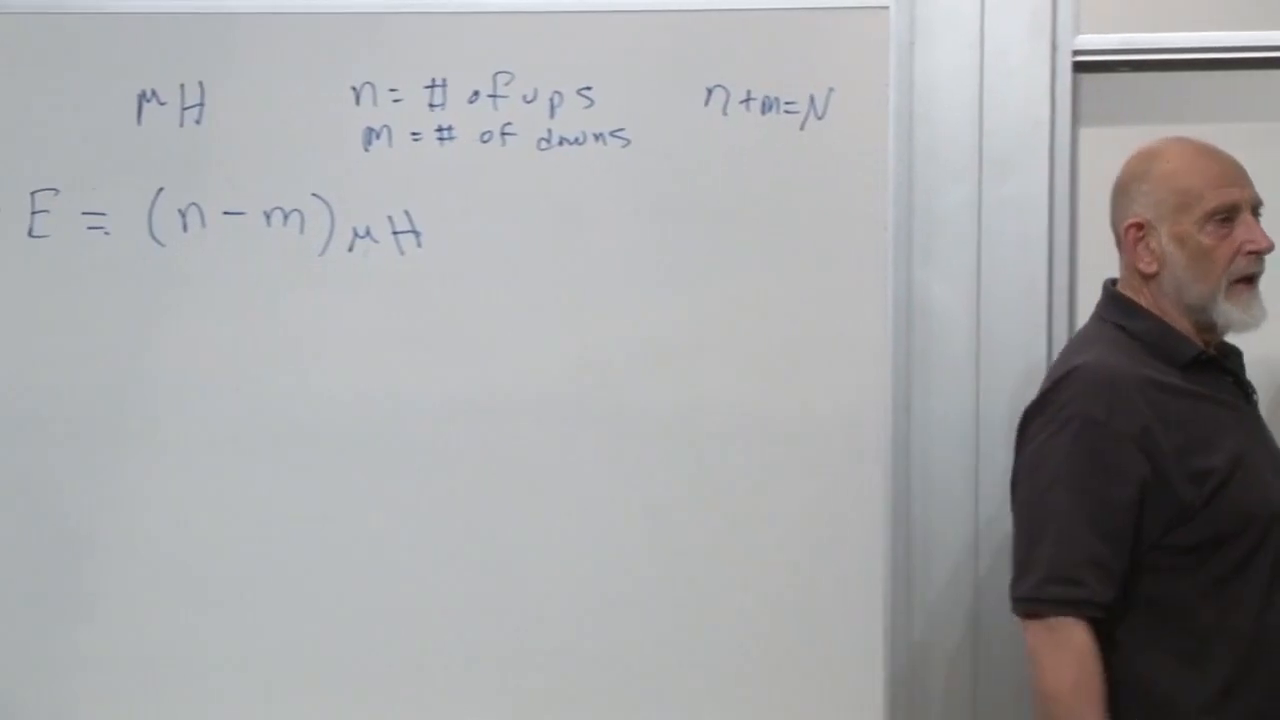
\includegraphics[width=0.90\textwidth]{lecture_08_figure_03.png}
\caption{独立自旋设置：\(n\)个向上自旋，\(m\)个向下自旋，\(n+m=N\)，以及\(E=(n-m)\mu H\)。}
\lectureframe{00:49:50}
\end{figure}

\begin{classroomqa}
\audiencequestion{\(H\)、\(\mu\)和\(E\)的量纲是什么？\(H\)是一个数还是磁场？}
\lecturerresponse{\(H\)表示外部施加的场强，\(\mu\)表示磁矩。它们的乘积\(\mu H\)具有能量的量纲。在抽象模型中，人们常将它们合并为一个能量值的参数，习惯上也用小写\(h\)表示。这里我们保留两个因子以显示其物理来源，而\(E\)是总能量。
\lecturetimestamp{00:48:21--00:49:27}}
\end{classroomqa}

\subsection{组态计数}

对于固定的\(n\)和\(m=N-n\)，选择\(N\)个格点中的哪\(n\)个向上。多重性为
\begin{equation}
 \Omega(n,m)=\binom{N}{n}
 =\frac{N!}{n!\,m!}.
 \label{eq:sm8-spin-multiplicity}
\end{equation}
这些组态中的每一个都具有相同的能量
\eqref{eq:sm8-counting-energy}。

\begin{classroomqa}
\audiencequestion{既然\(n\)和\(m\)并不独立，它们能同时作为求和指标吗？组合因子又出现在哪里？}
\lecturerresponse{它们可以写成一个受约束的对，满足\(n+m=N\)，或者可以对\(n=0,\ldots,N\)求和并令\(m=N-n\)。玻尔兹曼权重属于每一个单独的组态；将同一能量的所有组态归并在一起，会使该权重乘以\(N!/(n!\,m!)\)。
\lecturetimestamp{00:52:04--00:53:03}}
\end{classroomqa}

因此配分函数为
\begin{align}
 Z_N
 &=\sum_{n+m=N}
   \frac{N!}{n!\,m!}
   e^{-\beta\mu H(n-m)}
 \notag\\
 &=\sum_{n=0}^{N}
   \binom{N}{n}
   \left(e^{-\beta\mu H}\right)^n
   \left(e^{+\beta\mu H}\right)^{N-n}.
 \label{eq:sm8-spin-z-sum}
\end{align}
引入
\begin{equation}
 x=e^{-\beta\mu H},
 \qquad
 y=e^{+\beta\mu H}.
 \label{eq:sm8-xy}
\end{equation}
二项式定理随即完成计算：
\begin{align}
 Z_N
 &=\sum_{n=0}^{N}\binom{N}{n}x^n y^{N-n}
   =(x+y)^N
 \notag\\
 &=\left(e^{-\beta\mu H}+e^{+\beta\mu H}\right)^N
   =\left[2\cosh(\beta\mu H)\right]^N.
 \label{eq:sm8-spin-z-closed}
\end{align}

\begin{figure}[t]
\centering
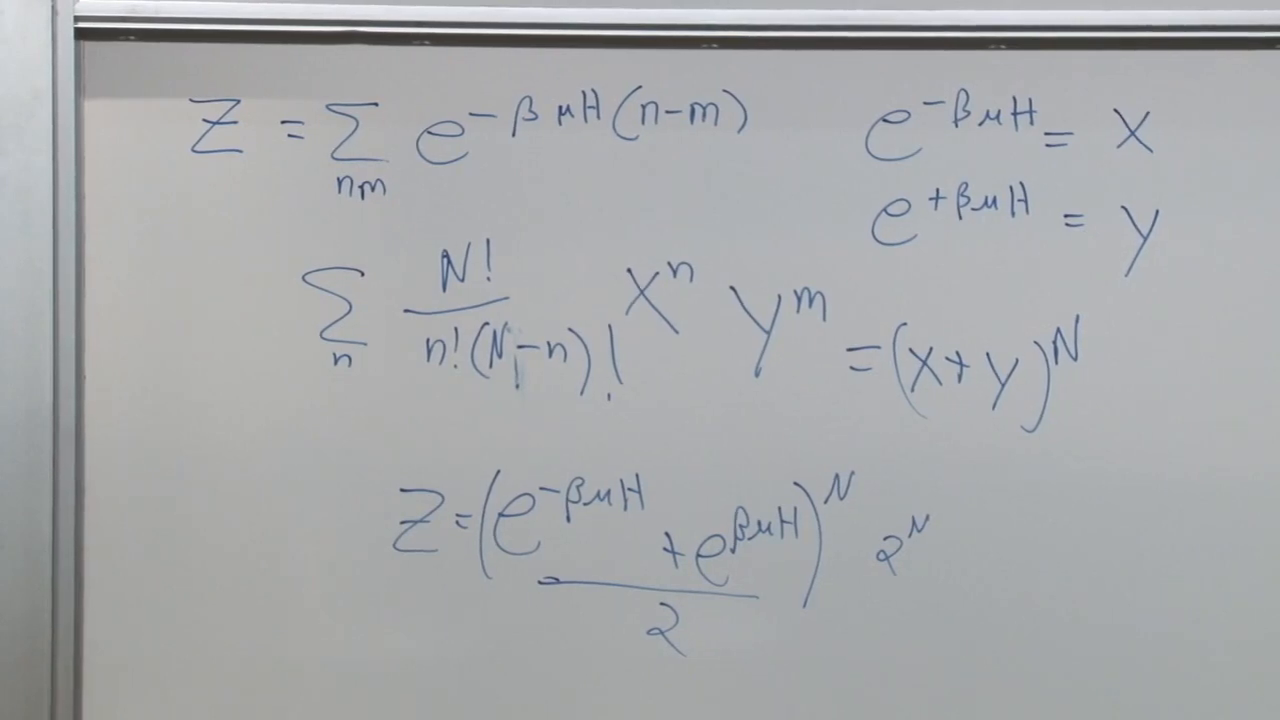
\includegraphics[width=0.90\textwidth]{lecture_08_figure_04.png}
\caption{配分函数求和、代换\(x\)和\(y\)，以及二项式约化为\(2\cosh(\beta\mu H)\)的幂。}
\lectureframe{00:56:00}
\end{figure}

还有一个更简短的推导。由于自旋是独立的，一个自旋有
\begin{equation}
 z_1=e^{-\beta\mu H}+e^{+\beta\mu H}
    =2\cosh(\beta\mu H),
 \label{eq:sm8-one-spin-z}
\end{equation}
以及\(Z_N=z_1^N\)。尽管如此，组合推导仍值得保留，因为它明确显示了多重性如何与能量竞争。

\section{组态磁化强度与系综磁化强度}

对于一个组态，定义其每格点的无量纲自旋过剩为
\begin{equation}
 M_{\rm conf}=\frac{n-m}{N}.
 \label{eq:sm8-config-magnetization}
\end{equation}
它的范围从全部自旋向上时的\(+1\)到全部自旋向下时的\(-1\)。这里使用的热力学磁化强度是其玻尔兹曼平均值，
\begin{equation}
 M=\left\langle M_{\rm conf}\right\rangle
  =\left\langle\frac{n-m}{N}\right\rangle.
 \label{eq:sm8-average-magnetization}
\end{equation}
因子\(\mu H\)不属于这个定义。它在计算过程中曾被短暂地写在那里，随后被去掉；\(\mu H\)将自旋过剩转换为能量。

逐组态地，
\begin{equation}
 E=N\mu H M_{\rm conf}.
 \label{eq:sm8-energy-config-m}
\end{equation}
求平均的线性性立即给出
\begin{equation}
 \langle E\rangle=N\mu H M.
 \label{eq:sm8-energy-average-m}
\end{equation}

\begin{figure}[t]
\centering
\includegraphics[width=0.90\textwidth]{lecture_08_figure_05.png}
\caption{自旋行、修正后的平均磁化强度，以及黑板上强调的能量关系。}
\lectureframe{01:01:22}
\end{figure}

\begin{classroomqa}
\audiencequestion{磁化强度是被赋予某个特定构型，还是我们在讨论平均磁化强度？为什么同样的关系对平均能量也成立？}
\lecturerresponse{两种概念都出现了，应当加以区分。\((n-m)/N\) 是一个构型中的取值；\(M\) 是它的玻尔兹曼平均。由于 \(E=N\mu H M_{\rm conf}\) 在每个构型中分别成立，用相同的概率对两边取平均便得到 \(\langle E\rangle=N\mu H M\)。固定量 \(N\)、\(\mu\) 和 \(H\) 穿过平均运算。
\lecturetimestamp{00:59:54--01:03:40}}
\end{classroomqa}

\begin{classroomqa}
\audiencequestion{这个模型如何能让每个自旋都沿北--南方向排列，而不偏向向上或向下？}
\lecturerresponse{没有东和西是两态模型本身所固有的；这是对允许自由度的限制。当前的外场模型 \emph{确实}在向上与向下之间有所偏向：按照我们的符号约定，外场降低向下自旋的能量。因此这个模型没有上--下对称性。下面引入的零场伊辛模型将恢复这种对称性。
\lecturetimestamp{01:03:41--01:04:53}}
\end{classroomqa}

\subsection{由配分函数求能量}

平均能量由通常的恒等式给出
\begin{equation}
 \langle E\rangle
 =-\frac{\partial}{\partial\beta}\log Z_N.
 \label{eq:sm8-energy-identity}
\end{equation}
利用 \eqref{eq:sm8-spin-z-closed}，
\begin{align}
 \log Z_N
 &=N\log 2+N\log\!\left[\cosh(\beta\mu H)\right],
 \notag\\
 \langle E\rangle
 &=-N\mu H\,
   \frac{\sinh(\beta\mu H)}{\cosh(\beta\mu H)}
 \notag\\
 &=-N\mu H\tanh(\beta\mu H).
 \label{eq:sm8-average-energy}
\end{align}
将其与 \eqref{eq:sm8-energy-average-m} 结合便得到
\begin{equation}
 \boxed{M=-\tanh(\beta\mu H)}.
 \label{eq:sm8-magnetization-tanh}
\end{equation}

答案的形状中蕴含着物理。回忆
\begin{equation}
 \cosh x=\frac{e^x+e^{-x}}{2},
 \qquad
 \sinh x=\frac{e^x-e^{-x}}{2}.
 \label{eq:sm8-hyperbolic-definitions}
\end{equation}
在原点附近，\(\tanh x=x+O(x^3)\)；对于大的正 \(x\)，它趋近于 \(1\)。由于 \(\beta=1/T\)，
\begin{equation}
 M\longrightarrow -1
 \quad (T\longrightarrow0),
 \qquad
 M\longrightarrow 0
 \quad (T\longrightarrow\infty).
 \label{eq:sm8-magnetization-limits}
\end{equation}
在零温下，每个自旋都占据能量较低的向下态。在无穷大温度下，所有构型都变得等权重，外场偏向被抹平。反转 \(H\) 会反转 \(M\)。

\begin{figure}[t]
\centering
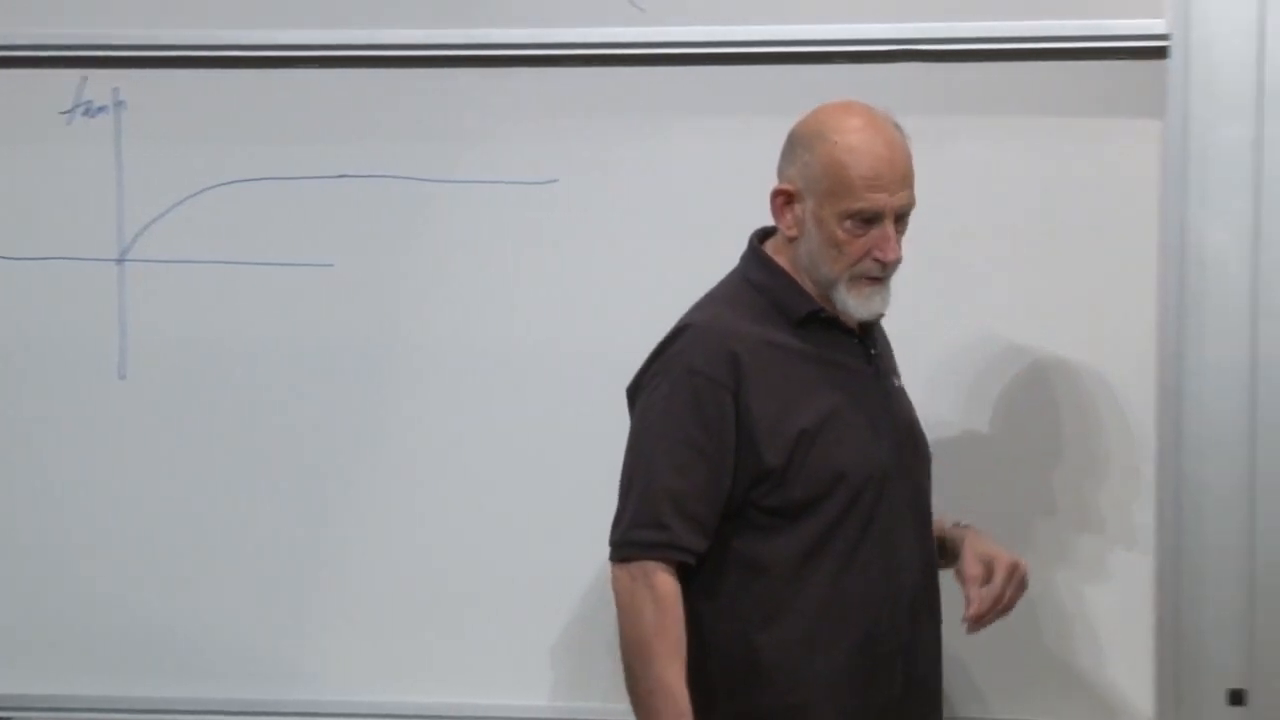
\includegraphics[width=0.90\textwidth]{lecture_08_figure_09.png}
\caption{双曲正切曲线在大的 \(\beta\mu H\) 下趋近于常数，并在原点附近呈线性。按照讲座的约定，物理磁化强度是所绘 \(\tanh\) 的负值。}
\lectureframe{01:13:14}
\end{figure}

\begin{classroomqa}
\audiencequestion{磁化强度连续变化。前面提到的相变温度在哪里？}
\lecturerresponse{在这个模型中没有相变温度。处于非零外场中的独立自旋太简单了，而且 \(\log Z_N=N\log[2\cosh(\beta\mu H)]\) 在每个有限正温度下都是光滑的。相变需要我们现在要接近的、有相互作用且对称的问题；二维零场伊辛模型是这一族中第一个具有有限温度相变的成员。
\lecturetimestamp{01:14:47--01:15:11}}
\end{classroomqa}

\section{伊辛模型：相邻对中的能量}

外场在统计开始之前就选定了一个方向。去掉这个场，让相邻自旋彼此提供有效场。如果某个格点的两个邻居都指向上，它们就偏向向上；如果两个都指向下，它们就偏向向下；如果一个指向上、一个指向下，那么在最简单的图像中它们的效果相互抵消。现在能量与对相关联，而不是与孤立格点相关联。

对于两个相邻自旋，取 \(J>0\) 并写出
\begin{equation}
 E_{12}=-J\sigma_1\sigma_2.
 \label{eq:sm8-pair-energy}
\end{equation}
取向一致的自旋有 \(\sigma_1\sigma_2=+1\) 和能量 \(-J\)；取向相反的自旋有乘积 \(-1\) 和能量 \(+J\)。因此，负号正是使该相互作用成为铁磁性的原因。

\begin{figure}[t]
\centering
\includegraphics[width=0.90\textwidth]{lecture_08_figure_06.png}
\caption{局域铁磁相互作用
\(E_{12}=-J\sigma_1\sigma_2\)。}
\lectureframe{01:19:59}
\end{figure}

在开放的一维链上，哈密顿量为
\begin{equation}
 {\cal H}=-J\sum_{i=1}^{N-1}\sigma_i\sigma_{i+1}.
 \label{eq:sm8-ising-chain-open}
\end{equation}
在周期性边界条件下，取 \(\sigma_{N+1}=\sigma_1\) 并对 \(N\) 求和。两种约定都把每个相邻对计数一次；对于长链，它们的边界差异变得可以忽略。

\begin{figure}[t]
\centering
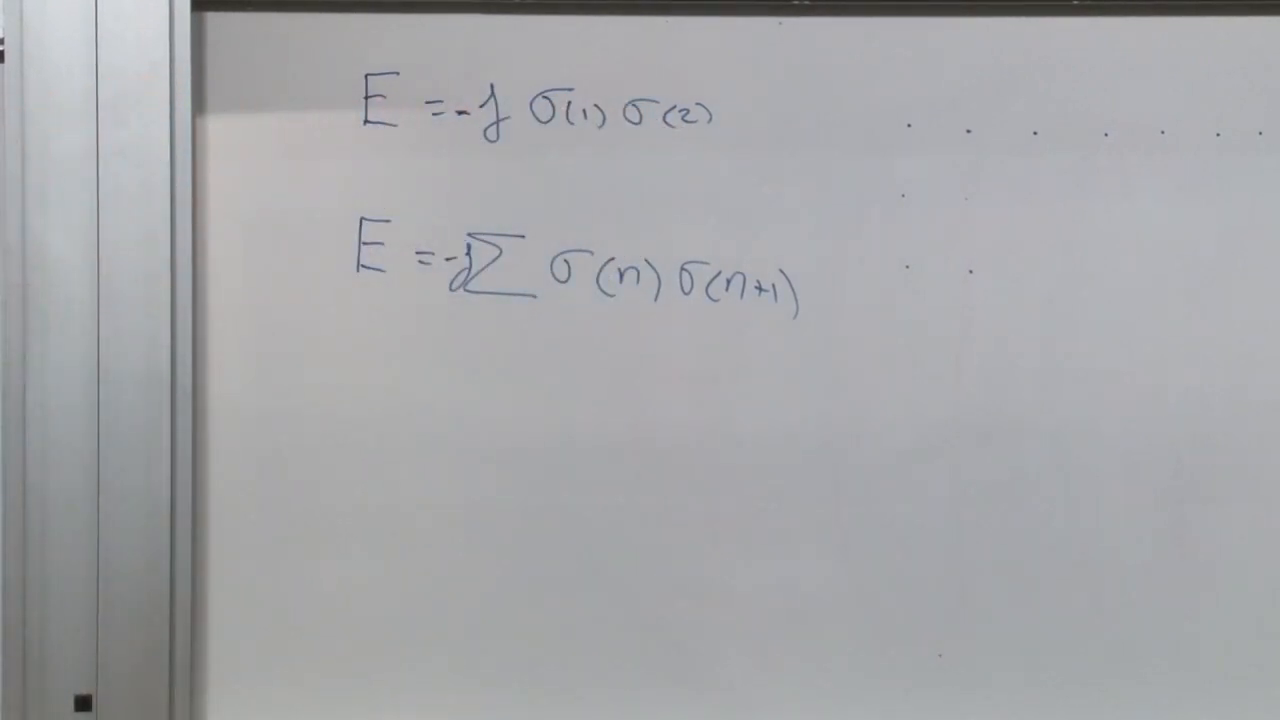
\includegraphics[width=0.90\textwidth]{lecture_08_figure_10.png}
\caption{局域对能量被推广到最近邻链哈密顿量。}
\lectureframe{01:20:46}
\end{figure}

在无穷大温度下，每个自旋串都等概率。平均而言，一半键取向一致，一半键取向相反，因此
\begin{equation}
 \left\langle\sigma_i\sigma_{i+1}\right\rangle_{T=\infty}=0,
 \qquad
 \left\langle{\cal H}\right\rangle_{T=\infty}=0.
 \label{eq:sm8-infinite-t-bond}
\end{equation}
这里的零能量并不是低能态。全部取向一致的基态每键能量为 \(-J\)，所以无穷大温度系综位于比它高出一个广延能量的位置。

\begin{classroomqa}
\audiencequestion{当每个单独的乘积 \(\sigma_i\sigma_{i+1}\) 要么是 \(+1\) 要么是 \(-1\) 时，平均乘积怎么会是零？}
\lecturerresponse{平均值不必是单个构型中所取的某个值。在无穷大温度下，取向一致和取向相反的键出现得同样频繁，因此它们的 \(+1\) 和 \(-1\) 贡献相互抵消。对磁化强度重要的那种平均区分在这里同样重要。
\lecturetimestamp{01:21:39--01:22:37}}
\end{classroomqa}

\subsection{两个基态与一个全局对称性}

在零温下，每个键都希望对齐。因此存在两个基态，
\begin{equation}
 (+,+,+,\ldots,+)
 \qquad\hbox{and}\qquad
 (-,-,-,\ldots,-).
 \label{eq:sm8-two-ground-states}
\end{equation}
它们具有完全相同的能量。哈密顿量使这一简并变得显而易见：翻转每一个自旋，
\begin{equation}
 \sigma_i\longmapsto-\sigma_i
 \qquad\hbox{for all }i,
 \label{eq:sm8-global-flip}
\end{equation}
每个键的乘积都保持不变，
\begin{equation}
 (-\sigma_i)(-\sigma_{i+1})
 =\sigma_i\sigma_{i+1}.
 \label{eq:sm8-global-flip-invariance}
\end{equation}
翻转单个自旋不是一种对称性，因为它会改变相邻键乘积的符号。翻转所有自旋才是一种对称性。这就是零场伊辛模型的全局\(\mathbb Z_2\)对称性。

\begin{figure}[t]
\centering
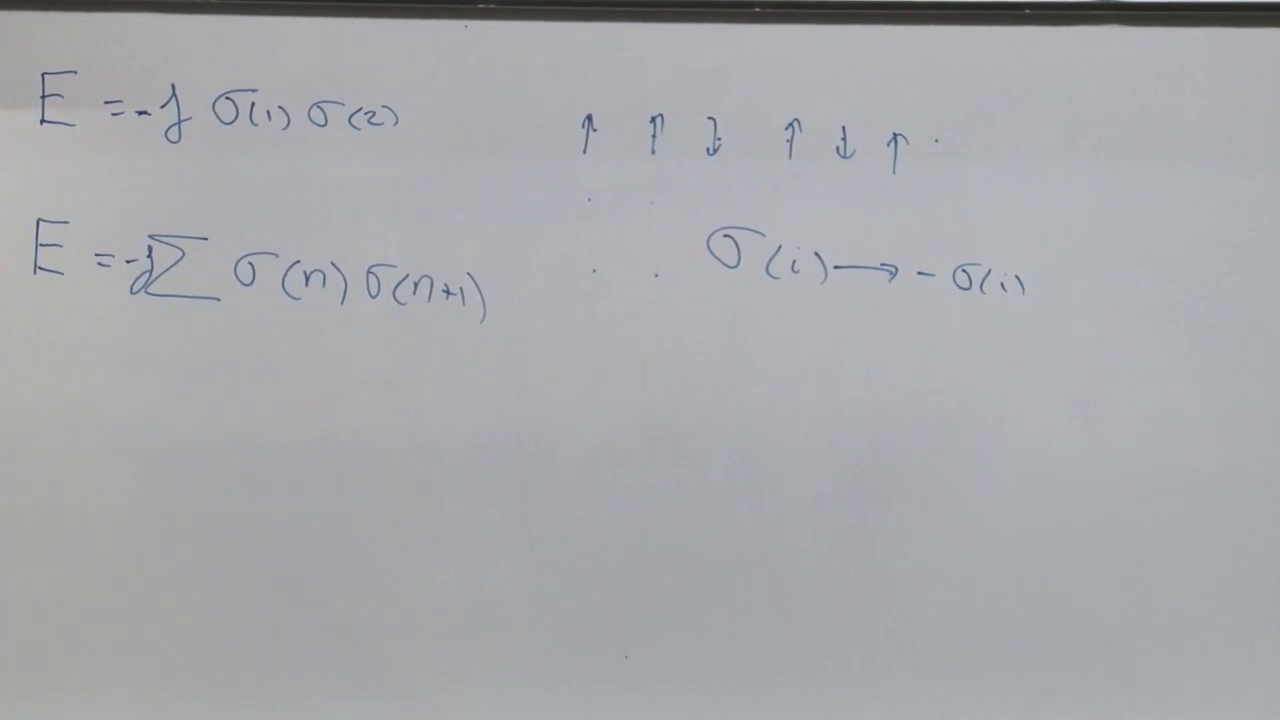
\includegraphics[width=0.90\textwidth]{lecture_08_figure_11.png}
\caption{链的哈密顿量与全局变换
\(\sigma_i\mapsto-\sigma_i\)并列，后者使每一对乘积保持不变。}
\lectureframe{01:26:31}
\end{figure}

在严格零温下对某一个自旋施加一个极微小的场。它打破两个基态之间的平局，而铁磁耦合将这一选择沿链传播开来。在态被选定之后撤去该场，一个大系统可以在极长的时间内保持其取向。这是通向自发对称性破缺的直观入口。

有一个本质性的统计限定。对于处于严格零场中的有限系统，正则系综给两个基态以相等的权重，因而平均磁化强度为零。破缺对称性的相是通过在撤去选择场之前先取热力学极限来定义的：
\begin{equation}
 M_*=\lim_{H\to0^+}\lim_{N\to\infty}M_N(H).
 \label{eq:sm8-order-of-limits}
\end{equation}
在一维最近邻模型中，这一极限仅在\(T=0\)处非零；任何有限温度都会破坏无限长链中的长程有序。在二维中，有序相在低于某个非零临界温度时仍然存在。

\subsection{一个历史性的更正}

课堂上的讲述在叙述这段历史时拿伊辛开了个玩笑。准确的年代顺序则更为友善。威廉·楞次提出了该模型，他的学生恩斯特·伊辛在其1924年的学位论文中求解了一维情形，该论文发表于1925年。伊辛正确地发现一维中不存在有限温度的鐵磁相变，尽管当时人们尚未理解更高维度的更广泛意义。克拉默斯与万尼尔发展了二维对偶性，并在1941年确定了方格点阵的临界点；昂萨格在1944年给出了著名的零场精确解。

接下来的计算现在已很明确。我们必须求出\eqref{eq:sm8-ising-chain-open}的配分函数，并确定其关联如何依赖于温度。该计算将明确显示为什么一维链没有有限温度相变，以及为什么维度至关重要。

\section{我们目前的进展}

回归问题与自旋问题是同一统计教训的两个版本。在气体中，熵的亏缺使一个宏观态以指数方式变得稀有：
\begin{equation}
 P(A)=e^{-\Delta S},
 \qquad
 \tau_{\rm rec}\sim\tau_{\rm mix}e^{\Delta S}.
 \label{eq:sm8-summary-recurrence}
\end{equation}
可逆力学允许回归，而巨大的相体积比解释了为什么日常经验只看到弛豫。剩下的时间箭头问题在于特殊的宇宙学初始条件，而不在于微观可逆性的失效。

对于场中的独立自旋，
\begin{equation}
 Z_N=\left[2\cosh(\beta\mu H)\right]^N,
 \qquad
 M=-\tanh(\beta\mu H).
 \label{eq:sm8-summary-spins}
\end{equation}
该系统明显是有偏置的，并随温度平滑变化。伊辛相互作用
\begin{equation}
 {\cal H}=-J\sum_i\sigma_i\sigma_{i+1}
 \label{eq:sm8-summary-ising}
\end{equation}
去除了外部偏置，恢复了全局上--下对称性，并提出了真正的有序化问题：一个对称的多体系统能否在非零温度下选择两个有序态之一？
